

\chapter{Perfect Secrecy}


	\section{Historical Context}
		\begin{itemize}
			\item Until World War 2 the design principles of ciphers were military secrets and not subject to open research
			\item During World War 2 especially the allies recruited many (civil) mathematicians and engineers in their cryptanalytic efforts
			\item It was realized that the central weaknesses of contemporary ciphers was that ciphertexts preserved certain properties/invariants of plaintext
			\begin{itemize}
				\item[->] E.g. Substitution Cipher: Ordered histogram of character frequencies was preserved
				\item[->] E.g. Enigma: We can rule out that a ciphertext encrypts a certain message
			\end{itemize}
			\item After WW2: Beginning of Information Age; Seminal works of Shannon ’48,’49
		\end{itemize}
		
	\section{Encryption Schemes (Shannon)}
		An encryption scheme consists of three algorithms: $(KeyGen,Enc,Dec)$ and three sets $\mathcal{K},\mathcal{M},\mathcal{C}$
		\begin{itemize}
			\item $KeyGen$: A randomized algorithm which outputs a key $K \in \mathcal{K}$
			\item $Enc(K,m)$: A randomized algorithm which takes a key $K \in \mathcal{K}$ and message $m \in \mathcal{M}$ as input and outputs a ciphertext $c \in \mathcal{C}$
			\item $Dec(K,c)$: A deterministic algorithm which takes as a key $K \in \mathcal{K}$ and a ciphertext $c \in \mathcal{C}$ as input 
			and outputs a message $m \in \mathcal{M}$
		\end{itemize}
	
	\section{Encryption Schemes: Correctness}
		\begin{itemize}
			\item An encryption scheme is called correct if it holds for all messages $m \in \mathcal{M}$ that
				$$Pr[Dec(K,Enc(K,m)) = m] = 1 \text{, where } K \leftarrow KeyGen()$$
			\item This probability is taken over all random choices involved, namely over the choice of the coins of $KeyGen$ and $Enc$
		\end{itemize}
	
	\section{Security}
		\begin{itemize}
			\item How do we define security?
			\item \textbf{Goal:} Security definition should guarantee that if the adversary sees a ciphertext, he shouldn't learn anything about the message
			\item \textbf{Idea:} Ciphertext should be independent of the message.
			\item What should the distribution of the message be? Any distribution!
		\end{itemize}
    
    
    
    \section{Perfect Secrecy: Part I}
	    \begin{definition}[Perfect Screcy 1]\label{Def.PerfectSecrecy1}
    		An encryption scheme $(KeyGen,Enc,Dec)$ is perfectly secret, if it holds for every random variable $M$ supported on the message space $\mathcal{M}$ that $M$ 
    		and $C=Enc(K,M)$ are independent, where $K$ is chosen by $K \leftarrow KeyGen()$.\newline
    	
		    I.e. it holds for all messages $m \in \mathcal{M}$ and every ciphertext $c \in \mathcal{C}$ with\\
		    $Pr[Enc(K,M)=c] > 0$ that
    		$$Pr[M=m \mid Enc(K,M) = c] = Pr[M=m]$$
   		 \end{definition}
   		 
   		 \subsection{One-Time Pad (OTP)}
   		 	\begin{center}
   		 		$\mathcal{K} = \mathcal{M} = \mathcal{C} = \{0,1\}^n$
   		 	\end{center}
   		 	\begin{itemize}
   		 		\item $KeyGen()$: Choose $K \leftarrow_{\$} \{0,1\}^n$ and output $K$
   		 		\item $Enc(K,m)$: Output $c \leftarrow K \oplus m$
   		 		\item $Dec(K,c)$: Output $m \leftarrow K \oplus c$
   		 		\item Note: Key as long as message!
   		 	\end{itemize}
   		 	
   		 	\begin{proof}[Correctness]
   		 		$Dec(K,c) = Dec(K,Enc(K,m)) = K \oplus K \oplus m = 0^n \oplus m = m$
   		 	\end{proof}
   		 
   		 \subsection{One-Time Pad: Perfect Secrecy}
   		 	\begin{itemize}
   		 		\item $K \leftarrow_{\$} \{0,1\}^n$ and $K \oplus m$ is uniformly random
   		 		\item $M$ supported of $\mathcal{M}$, with $M$ and $K$ are independent
   		 		\item $M \oplus K$ is distributed uniformly random
   		 	\end{itemize}
   		 	Fix any distribution $M$, and show that for all $m,c$:
   		 	$$Pr[M=m \mid Enc(K,M)=c] = Pr[M=m]$$
   		 	\begin{proof}
	   		 	\begin{align*}
   			 		Pr[M=m \mid Enc(K,M)=c] &= Pr[M=m \mid K \oplus M = c]\\
   			 		&= \frac{Pr[K \oplus M = c \mid M=m] \cdot Pr[M=m]}{Pr[K \oplus M =c]} \text{(Baye's Rule)}
   			 	\end{align*}
   			 	Let's consider $Pr[K \oplus \mid M=m]$:
   			 	\begin{align*}
   			 		Pr[K \oplus \mid M=m] &= Pr[K \oplus M = c]\\
   			 		&= \sum\limits_{m'} Pr[K \oplus M = c \mid M = m'] \cdot Pr[M=m']\\
   			 		&= \sum\limits_{m'} \frac{1}{2^n} \cdot Pr[M=m']\\
   			 		&= \frac{1}{2^n} \cdot \sum\limits_{m'} Pr[M=m'] = \frac{1}{2^n}
   			 	\end{align*}
   			 	So it follows that
   			 	$$Pr[M=m \mid K \oplus M = c] = \frac{\frac{1}{2^n} \cdot Pr[M=m]}{\frac{1}{2^n}} = \frac{\frac{1}{2^n}}{\frac{1}{2^n}} \cdot Pr[M=m] = Pr[M=m]$$
   		 	\end{proof}
   		 
   		 \subsection{One-Time Pad in any Finite Group}
   		 	\begin{center}
   		 		$\mathcal{K} = \mathcal{M} = \mathcal{C} = G$
   		 	\end{center}
   		 	\begin{itemize}
   		 		\item $KeyGen()$: Choose $K \leftarrow_{\$} G$ and output $K$
   		 		\item $Enc(K,m)$: Output $c \leftarrow K \oplus m$
   		 		\item $Dec(K,c)$: Output $m \leftarrow K^{-1} \oplus c$
   		 	\end{itemize}
   		 
   		 \subsection{Why "One-Time Pad"?}
   		 	\begin{itemize}
   		 		\item Invented by Vernam in 1917
   		 		\item Proven secure by Shannon in 1949
   		 		\item The proof of security only holds if the key is used at most once
   		 		\item If the key is reused, this essentially becomes a Vigenere cipher!
   		 		\item Thus, the OTP consumes large amounts of key material
   		 		\item Can we do better?
   		 	\end{itemize}
	
	\section{Summary 1}
		\begin{itemize}
			\item We defined the syntax and the correctness property for encryption schemes
			\item We provided a definition of perfect security which captures the intuition that ciphertexts should reveal no information about the plaintext
			\item We showed that the one time pad is perfectly secret
		\end{itemize}
	
	
	
	\section{Discussion: Perfect Secrecy}
		\begin{itemize}
			\item This definition (\cref{Def.PerfectSecrecy1}) is \textbf{not easy to work with} when designing larger protocols
			\item Also, it does not immediately generalize to "weaker" security notions that allow for more efficient schemes.
			\item Another Approach: In the context of historic ciphers, we also have seen distinguishing attacks
			\item The adversary knows that a ciphertext encrypts one out of two messages and has to find out which one it is
			\item Is this a minimal attack goal?
		\end{itemize}
    
    
    
    \section{Perfect Secrecy: Part II}
    	\begin{definition}[Perfect Secrecy 2]\label{Def.PerfectSecrecy2}
    		An encryption scheme $(KeyGen,Enc,Dec)$ is perfectly secret, if it holds for all $m,m' \in \mathcal{M}$ and all $c \in \mathcal{C}$ that
    		$$Pr[Enc(K,m)=c] = Pr[Enc(K,m')=c]$$
    		where $K \leftarrow KeyGen()$
    	\end{definition}
    	
    	\subsection{Discussion}
    		\begin{itemize}
    			\item The definitions of perfect secrecy provided so far (1 $\&$ 2) only concerned the distributions of messages and ciphertexts
    			\item There is no explicit mention of an adversary in these definitions
    			\item Recall from Lecture 1.3 that we want to study security notions against adversaries with different resources
    			\item Let’s make the adversary explicit
    		\end{itemize}

		\begin{definition}[Perfect Screcy 3]\label{Def.PerfectSecrecy3}
    		We first define some expressions:
        		\begin{itemize}
        			\item Let $(KeyGen,Enc,Dec)$ be an encryption scheme
            		\item Let $\mathcal{A}$ be a (possibly unbounded) randomized algorithm, called the adversary
            		\item Let $IND_{\mathcal{A}}$ be a random variable which describes the output of the challenger at the end of the experiment
            		\item Consider this experiment:
        		\end{itemize}
        		\begin{center}
					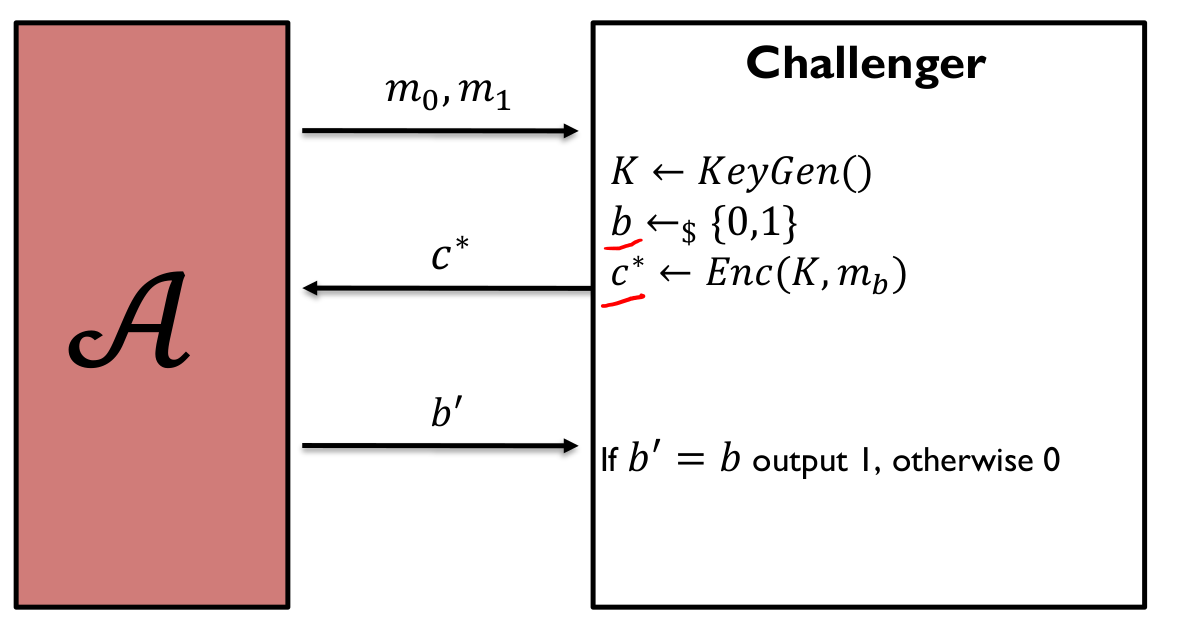
\includegraphics[width=120mm]{Graphics/Perfect Secrecy/def3.png}\newline
				\end{center}
				\begin{itemize}
					\item We call this the ciphertext indistinguishability experiment
				\end{itemize}
    
    	An encryption scheme $(KeyGen,Enc,Dec)$ is perfectly secret, if it holds for \textbf{every adversary} $\mathcal{A}$ that
    	$$Pr[IND_{\mathcal{A}} = 1] = \frac{1}{2}$$
   		where the probability is taken over all random choices of the experiment.\newline
    	\end{definition}
    	
    	\begin{theorem}
    		\cref{Def.PerfectSecrecy1}, \cref{Def.PerfectSecrecy2} and \cref{Def.PerfectSecrecy3} of perfect secrecy are equivalent.
    	\end{theorem}
    	\begin{proof}
    		Proof concept: $((2) \Rightarrow (1)) \rightarrow ((3) \Rightarrow (2)) \rightarrow ((1) \Rightarrow (3))$
    		\begin{itemize}
    			\item[$(2) \Rightarrow (1)$] For all $m,m',c$ show
    					$$Pr[Enc(K,m)=c] = Pr[Enc(K,m')=c] \Rightarrow \delta_{c} := Pr[Enc(K,m)=c]$$
    				Let $M$ be a distribution of messages.
    				Need to show for all $m,c$ that
    					$$Pr[M=m \mid Enc(K,M)=c] = Pr[M=m]$$
    				With Baye's rule it follows, that
    					$$Pr[M=m \mid Enc(K,M)=c] = \frac{Pr[Enc(K,M)=c \mid M=m] \cdot Pr[M=m]}{Pr[Enc(K,M)=c]}$$
    				Now we consider the changed conditional probability
    					$$Pr[Enc(K,M)=c \mid M=m] = Pr[Enc(K,m)=c \mid M=m] = Pr[Enc(K,m)=c] = \delta_c$$
    				The denominator can be formed as follows
    				\begin{align*}
    					Pr[Enc(K,M)=c] &= \sum\limits_{m' \in Supp(M)} Pr[Enc(K,m')=c \mid M=m'] \cdot Pr[M=m']\\
    					&= Pr[Enc(K,m')=c] \cdot \sum\limits_{m' \in Supp(M)} Pr[M=m']\\
    					&= \delta_c \cdot \sum\limits_{m' \in Supp(M)} Pr[M=m'] = \delta_c
					\end{align*}
					So it follows 
					$$Pr[M=m \mid Enc(K,M)=c] = \frac{\delta_c \cdot Pr[M=m]}{\delta_c} = Pr[M=m]$$
					
    			\item[$(3) \Rightarrow (2)$] Via contraposition:\\
    				Assume \cref{Def.PerfectSecrecy2} does not hold, i.e. there exist $m,m',c$ so that
    					$$Pr[Enc(K,m)=c] > Pr[Enc(K,m')=c]$$
    				\textbf{Strategy:} Construct $\mathcal{A}$ so that $Pr[IND_{\mathcal{A}}=1] > \frac{1}{2}$
    				\begin{center}
						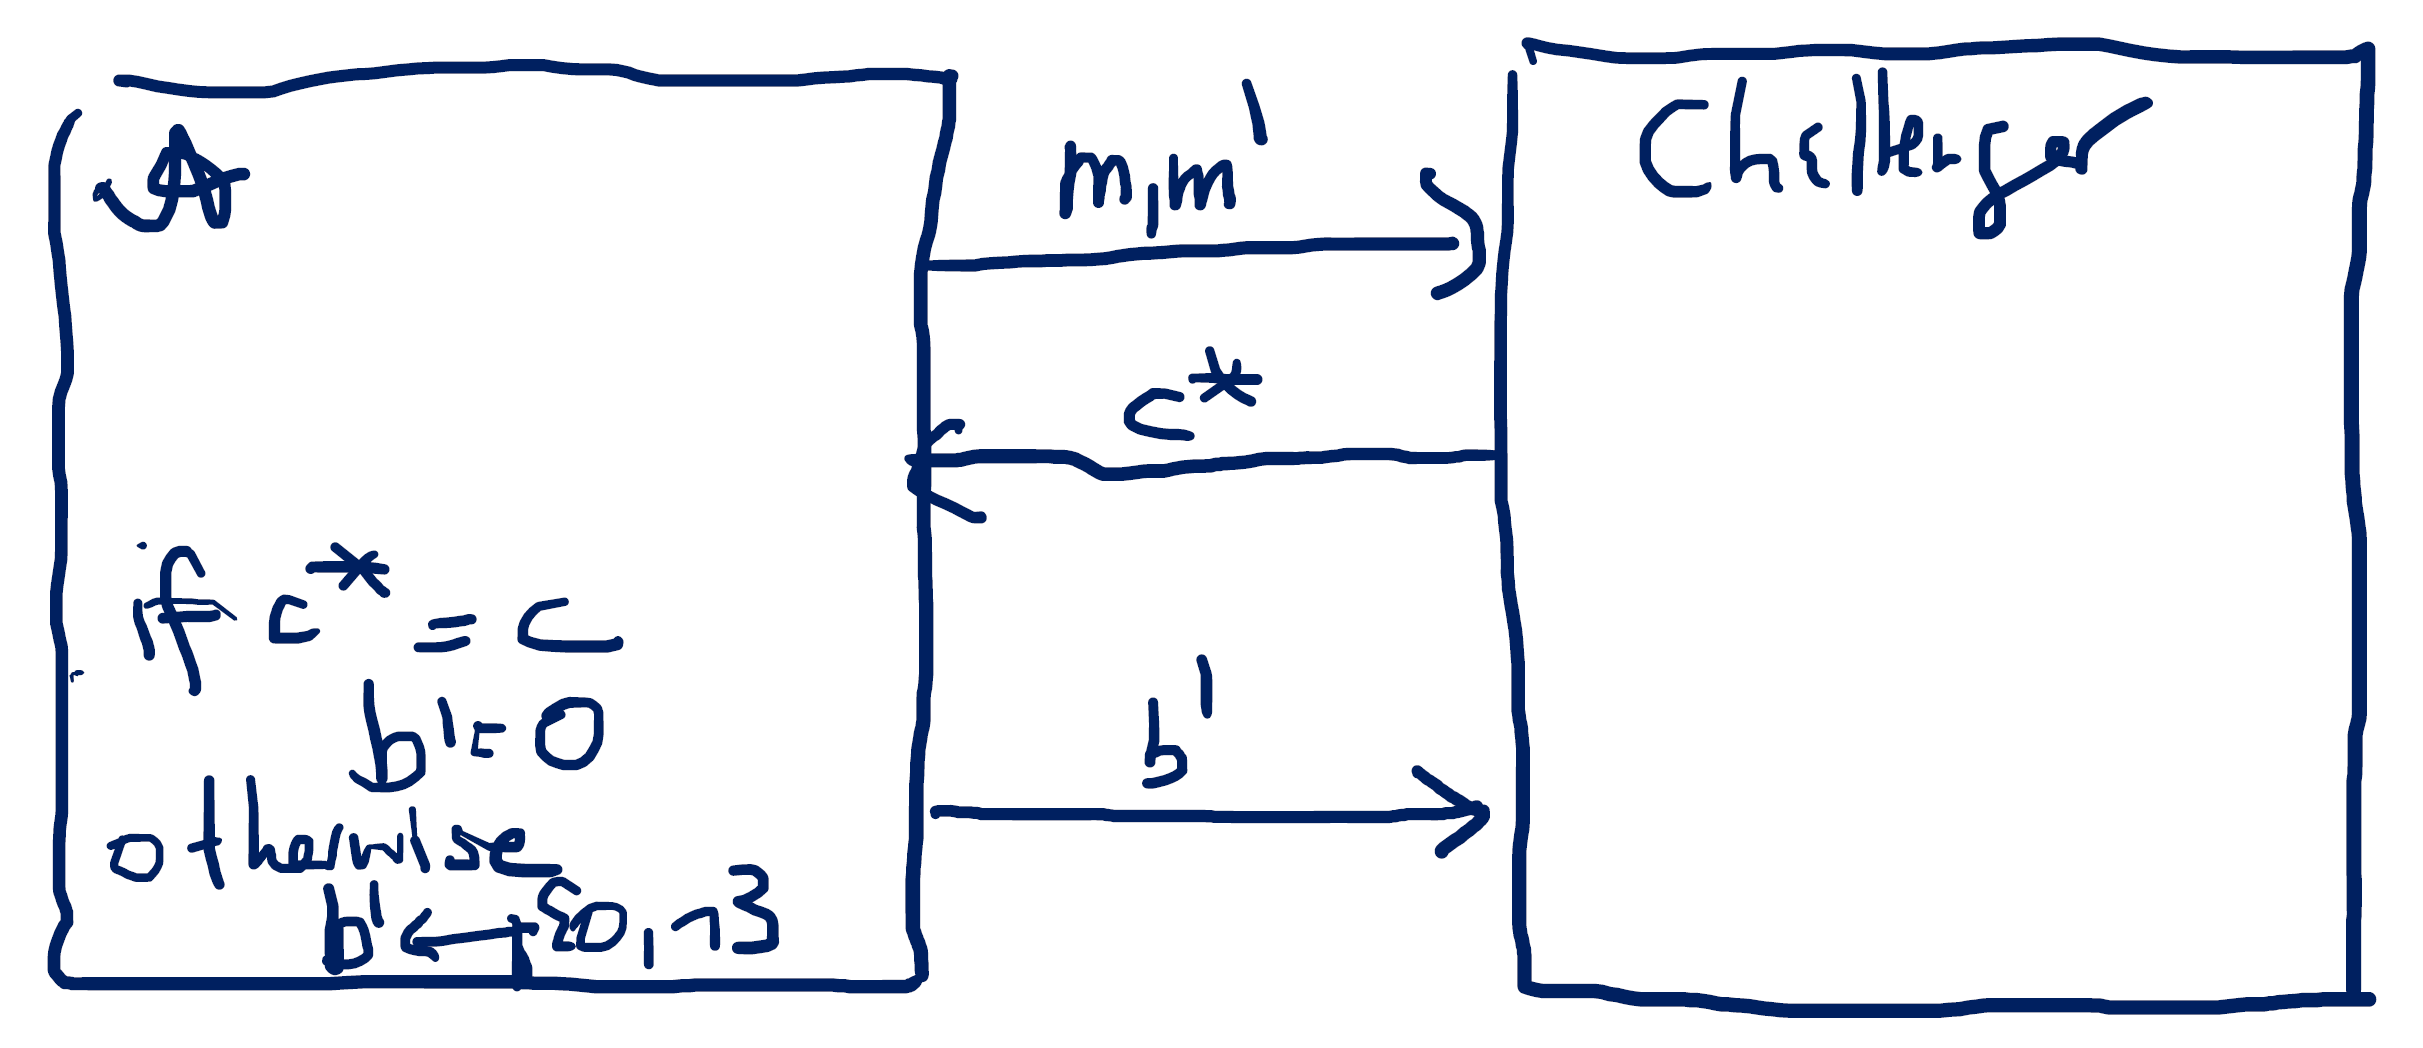
\includegraphics[width=120mm]{Graphics/Perfect Secrecy/Proof(3)to(2).png}\newline
					\end{center}
					with $Pr[c^* = c] > 0$
						$$Pr[Enc(K,m)=c] > Pr[Enc(K,m')=c] \geq 0$$
					With the "law of total probability" it follows that
						$$Pr[IND_{\mathcal{A}}=1] = Pr[IND_{\mathcal{A}}=1 \mid c^*=c] \cdot Pr[c^* = c] + Pr[IND_{\mathcal{A}}=1 \mid c^* \neq c] \cdot Pr[c^* \neq c]$$
					Now we need to show that $Pr[IND_{\mathcal{A}}=1 \mid c^*=c]$:\\
					If $c^* = c$ it holds that $IND_{\mathcal{A}}=1$ if and only if $b=0$\\
					Wherever $c^* = c$ adversary $\mathcal{A}$ will guess $b' = 0$ (by construction)\\
					$\Rightarrow$ Under the condition $c^* = c$ the events $IND_{\mathcal{A}}=1$ and $b=0$ are equivalent.
						$$Pr[IND_{\mathcal{A}}=1 \mid c^* = c] = Pr[b=0 \mid c^* = c]$$
					We will compute $Pr[b=0 \mid c^* = c]$ using Baye's rule and LOTP
						$$Pr[b=0 \mid c^* = c] = \frac{Pr[c^* = c \mid b=0] \cdot Pr[b=0]}{Pr[c^* = c]}$$
					We have to compute two things, first
					\begin{align*}
						Pr[c^* = c \mid b=0] = Pr[Enc(K,m)=c]
					\end{align*}
					and then
					\begin{align*}
						Pr[c^* = c] &= Pr[c^* = c \mid b=0] \cdot Pr[b=0] + Pr[c^* = c \mid b=1] \cdot Pr[b=1]\\
						&= Pr[Enc(K,m)=c] \cdot \frac{1}{2} + Pr[Enc(K,m')=c] \cdot \frac{1}{2}\\
						&= \frac{1}{2} \cdot (Pr[Enc(K,m)=c] + Pr[Enc(K,m')=c])
					\end{align*}
					Now we want to use the results:
					\begin{align*}
						Pr[b=0 \mid c^* = c] &= \frac{Pr[Enc(K,m)=c] \cdot \frac{1}{2}}{\frac{1}{2} \cdot (Pr[Enc(K,m)=c] + Pr[Enc(K,m')=c])}\\
						&= \frac{1}{1 + \frac{Pr[Enc(K,m')=c]}{Pr[Enc(K,m)=c]}} > \frac{1}{2}
					\end{align*}
					with $\frac{Pr[Enc(K,m')=c]}{Pr[Enc(K,m)=c]} < 1$
					
				\item[$(1) \Rightarrow (3)$]
					Let $\mathcal{A}$ be an adversary for the $IND$ experiment.\\
					For now assume that $\mathcal{A}$ is deterministic.
					$\mathcal{A}$ always uses some messages $m_0,m_1$
    				\begin{center}
						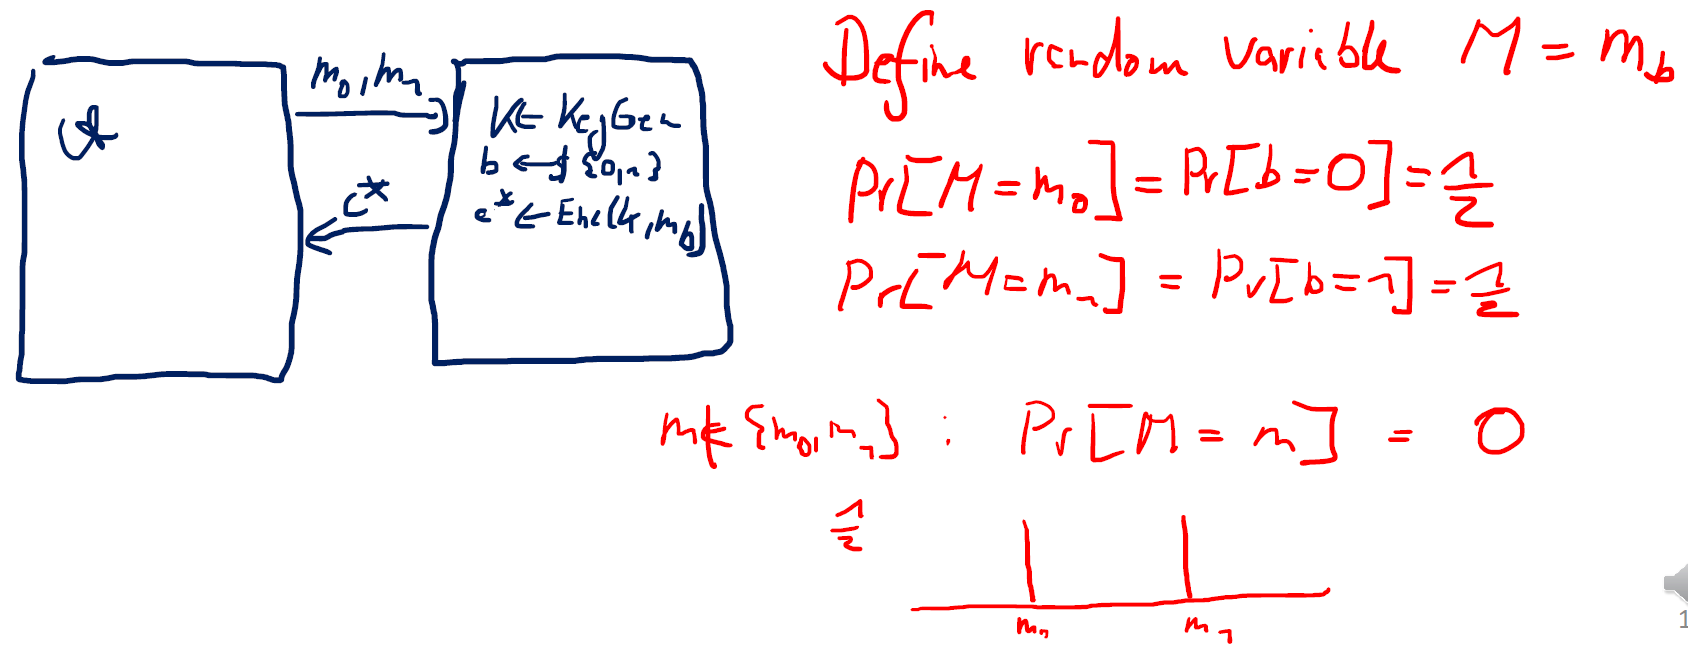
\includegraphics[width=120mm]{Graphics/Perfect Secrecy/Proof(1)to(3).png}\newline
					\end{center}
					So $c^* = Enc(K,m_b) = Enc(K,M)$\\
					\underline{Idea:} Use \cref{Def.PerfectSecrecy1} to show that $c^*$ is independent of $M$ and therefore of $b$\\
					\underline{First:} For $\beta \in \{0,1\}$ the events $M = m_{\beta}$ are equivalent.\\
					For all ciphertexts $c$ it holds:
						$$Pr[b = \beta \mid c^* = c] = Pr[M = m_{\beta} \mid Enc(K,M)=c] = Pr[M = m_{\beta}] = \frac{1}{2}$$
					If we recall that $\mathcal{A}$ is deterministic, we can follow that $b' = b'(c^*)$ is a deterministic function of $c^*$.
					\begin{align*}
						Pr[IND_{\mathcal{A}} = 1] &= Pr[b = b'(c^*)]\\
						&= \sum\limits_{c \in \mathcal{C}} Pr[b = b'(c^*) \mid c^* = c] \cdot Pr[c^* = c] \text{, with LOTP}\\
						&= \sum\limits_{c \in \mathcal{C}} Pr[b = b'(c) \mid c^* = c] \cdot Pr[c^* = c]\\
						&= \sum\limits_{c \in \mathcal{C}} \frac{1}{2} \cdot Pr[c^* = c] = \frac{1}{2} \cdot \sum\limits_{c \in \mathcal{C}} Pr[c^* = c]\\
						&= \frac{1}{2} \cdot 1 = \frac{1}{2}
					\end{align*}
					But what about randomized $\mathcal{A}$?\\
					$\mathcal{A}$ takes as input additional random coins $r \leftarrow \{0,1\}^l$ and write as $\mathcal{A}(r)$ to make this explicit.\\
					\underline{Idea:} For every fixed $\delta \in \{0,1\}^l$, $\mathcal{A}(\delta)$ is a deterministic algorithm.\\
					That means $Pr[IND_{\mathcal{A}(\delta)} = 1] = \frac{1}{2}$ (*), and it follows with the LOTP that
					\begin{align*}
						Pr[IND_{\mathcal{A}(r)} = 1] &= \sum\limits_{\delta \in \{0,1\}^l} Pr[IND_{\mathcal{A}(\delta)} = 1 \mid r = \delta] \cdot Pr[r = \delta]\\
						&= \sum\limits_{\delta \in \{0,1\}^l} \frac{1}{2} \cdot Pr[r = \delta] \text{, because of (*)}\\
						&= \frac{1}{2} \cdot \sum\limits_{\delta \in \{0,1\}^l} Pr[r = \delta] = \frac{1}{2} \cdot 1 = \frac{1}{2}
					\end{align*}

    		\end{itemize}
    	\end{proof}

	
    \begin{itemize}
    	\item For the one time pad, keys are as large as the message and can only be use once.
    	\item Can we construct perfectly secret encryption with short(er) keys? $\leftarrow$ No!
    \end{itemize}
    
    \begin{theorem}[Shannon's Theorem]
        Let $(KeyGen,Enc,Dec)$ be an encryption scheme with key space $\mathcal{K}$,message space $\mathcal{M}$ and ciphertext space $\mathcal{C}$. If it is perfectly secure, then 
        $$\vert \mathcal{K} \vert \geq \vert \mathcal{M} \vert$$
    \end{theorem}
    \begin{proof}
    	Assume $|\mathcal{K}| < |\mathcal{M}|$\\
    	\underline{Strategy:} Show there exist $m_0,m_1$ and ciphertext $c$ so that
    		$$Pr[Enc(K,m_0) = c] > 0$$
    		$$Pr[Enc(K,m_1) = c] = 0$$
    	This contradicts \cref{Def.PerfectSecrecy2} of perfect secrecy.\\
    	
    	Fix an arbitrary $m_0 \in \mathcal{M}$, a key $K_0 \in \mathcal{K}$, and set
    		$$c = Enc(K_0,m_0)$$
    	Define the set
    		$$S = \{ Dec(k,c) \mid k \in \mathcal{K} \} \subseteq \mathcal{M}$$
    	$\Rightarrow |S| \leq |\mathcal{K}| < |\mathcal{M}|$\\
    	$\Rightarrow \mathcal{M} \backslash S \neq \emptyset$, i.e. there exist $m_1 \in \mathcal{M} \backslash S$\\
    	
    	We claim there exists no key $K \in \mathcal{K}$ s.t. $c = Enc(K,m_1)$.\\
    	If there was such a $K$, then by correctness of the scheme it holds
    		$$Dec(K,c) = Dec(K,Dec(K,m_1)) = m_1$$
    	$\Rightarrow m_1 \in S$\\
    	Contradiction to the given condition that $m_1 \in \mathcal{M} \backslash S$
    \end{proof}
    
    \section{Summary 2}
    	\begin{itemize}
    		\item Two alternate definitions for perfect secrecy.
    		\item All 3 definitions are equivalent.
    		\item Perfectly secret schemes have keys as large as the message which can only be used once.
    	\end{itemize}
    
    
    \newpage
    
    
    
    
    
    
    
    
    
    
    
    
    
    
    
    
    
    
    
    
    
    
    
    
    
    
    
    
    
    